\chapter{Plotting}\label{plotting}

This chapter presents ways to create figures and graphs, more generally
called \textbf{data visualizations}. As examples, we'll generate three
figures:

\begin{itemize}
\item
  We'll replicate a figure from the Pew Research Center that shows
  changes in religious affiliation in the United States over time.
\item
  We'll replicate a figure from \emph{The Economist} that shows the
  prices of sandwiches in Boston and London (we saw this data back in
  Chapter 3).
\item
  We'll make a plot to test Zipf's law, which describes the relationship
  between word frequencies and their ranks.
\end{itemize}

With the tools in this chapter, you can generate a variety of simple
graphs. We will see more visualization tools in later chapters. But
before we get started with plotting, we need a new feature: keyword
arguments.

\section{Keyword Arguments}\label{keyword-arguments}

When you call most functions, you have to provide values. For example,
when you call \passthrough{\lstinline!np.exp!}, you provide a number.

\begin{lstlisting}[language=Python,style=source]
import numpy as np

np.exp(1)
\end{lstlisting}

\begin{lstlisting}[style=output]
2.718281828459045
\end{lstlisting}

\pagebreak

When you call \passthrough{\lstinline!np.power!}, you provide two
numbers.

\begin{lstlisting}[language=Python,style=source]
np.power(10, 6)
\end{lstlisting}

\begin{lstlisting}[style=output]
1000000
\end{lstlisting}

The values you provide are called \textbf{arguments}. Specifically, the
values in these examples are \textbf{positional arguments} because their
position determines how they are used. In the second example,
\passthrough{\lstinline!power!} computes \passthrough{\lstinline!10!} to
the sixth power, not \passthrough{\lstinline!6!} to the tenth power --
because of the order of the arguments.
\index{argument}
\index{keyword argument}
\index{positional argument}

Many functions also take \textbf{keyword arguments}, which are
identified by name. For example, we have previously used
\passthrough{\lstinline!int!} to convert a string to an integer. Here's
how we use it with a string as a positional argument:

\begin{lstlisting}[language=Python,style=source]
int('21')
\end{lstlisting}

\begin{lstlisting}[style=output]
21
\end{lstlisting}

By default, \passthrough{\lstinline!int!} assumes that the number is in
base 10. But you can provide a keyword argument that specifies a
different base. For example, the string \passthrough{\lstinline!'21'!},
interpreted in base 8, represents the number
\passthrough{\lstinline!2 * 8 + 1 = 17!}. Here's how we do this
conversion using \passthrough{\lstinline!int!}.

\begin{lstlisting}[language=Python,style=source]
int('21', base=8)
\end{lstlisting}

\begin{lstlisting}[style=output]
17
\end{lstlisting}

The integer value \passthrough{\lstinline!8!} is a keyword argument,
with the keyword \passthrough{\lstinline!base!}. Specifying a keyword
argument looks like an assignment statement, but it does not create a
new variable. And when you provide a keyword argument, you don't choose
the variable name -- it is specified by the function. If you provide a
name that is not specified by the function, you get an error.
\index{TypeError}

\begin{lstlisting}[language=Python,style=source]
%%expect TypeError

int('123', bass=11)
\end{lstlisting}

\begin{lstlisting}[style=output]
TypeError: 'bass' is an invalid keyword argument for int()
\end{lstlisting}

\textbf{Exercise:} The \passthrough{\lstinline!print!} function takes a
keyword argument called \passthrough{\lstinline!end!} that specifies the
character it prints at the end of the line. By default,
\passthrough{\lstinline!end!} is the newline character,
\passthrough{\lstinline!\\n!}.

\pagebreak

So if you call \passthrough{\lstinline!print!} more than once, the outputs normally appear on separate lines, like this:

\begin{lstlisting}[language=Python,style=source]
for x in [1, 2, 3]:
    print(x)
\end{lstlisting}

\begin{lstlisting}[style=output]
1
2
3
\end{lstlisting}

Modify the previous example so the outputs appear on one line with
spaces between them. Then modify it to print an open bracket at the
beginning and a close bracket and newline at the end.

\section{Graphing Religious
Affiliation}\label{graphing-religious-affiliation}

Now we're ready to make some graphs. In October 2019 the Pew Research
Center published ``In U.S., Decline of Christianity Continues at Rapid
Pace''. It includes this figure, which shows changes in religious
affiliation among adults in the U.S. over the previous 10 years.

As an exercise, we'll replicate this figure. It shows results from two
sources, Religious Landscape Studies and Pew Research Political Surveys.
The political surveys provide data from more years, so we'll focus on
that.

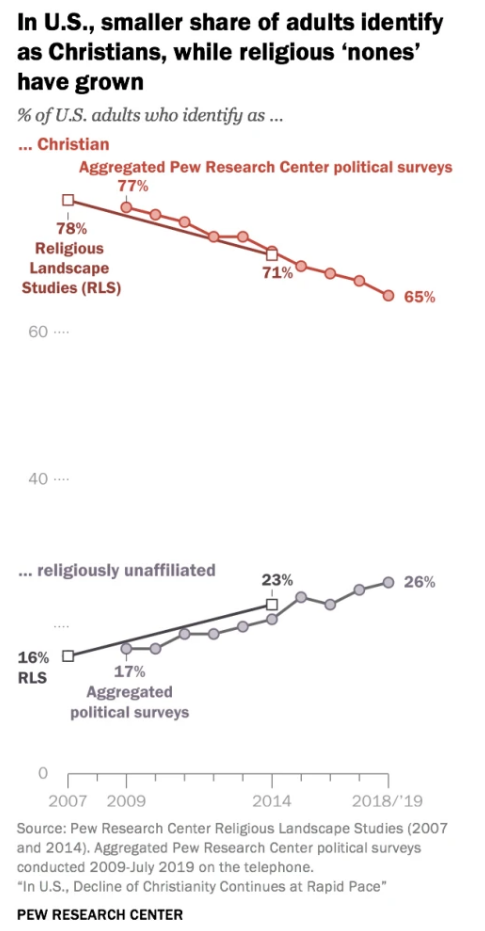
\includegraphics[scale=0.3]{figs/pew_religion_figure1.png}

The data from the figure are available from Pew Research, but they are
in a PDF document. It is sometimes possible to extract data from PDF
documents, but for now we'll enter the data by hand.
\index{Pew Research}

\begin{lstlisting}[language=Python,style=source]
year = [2009, 2010, 2011, 2012, 2013, 2014, 2015, 2016, 2017, 2018]
\end{lstlisting}

\begin{lstlisting}[language=Python,style=source]
christian = [77, 76, 75, 73, 73, 71, 69, 68, 67, 65]
\end{lstlisting}

\begin{lstlisting}[language=Python,style=source]
unaffiliated = [17, 17, 19, 19, 20, 21, 24, 23, 25, 26]
\end{lstlisting}

The library we'll use for plotting is Matplotlib -- more specifically,
we'll use a part of it called Pyplot, which we'll import with the
shortened name \passthrough{\lstinline!plt!}.
\index{Matplotlib}
\index{Pyplot}

\begin{lstlisting}[language=Python,style=source]
import matplotlib.pyplot as plt
\end{lstlisting}

Pyplot provides a function called \passthrough{\lstinline!plot!} that
makes a line plot. It takes two sequences as arguments, the
\passthrough{\lstinline!x!} values and the \passthrough{\lstinline!y!}
values. The sequences can be tuples, lists, or arrays.
\index{plot (Pyplot function)}

\begin{lstlisting}[language=Python,style=source]
plt.plot(year, christian);
\end{lstlisting}

\begin{center}
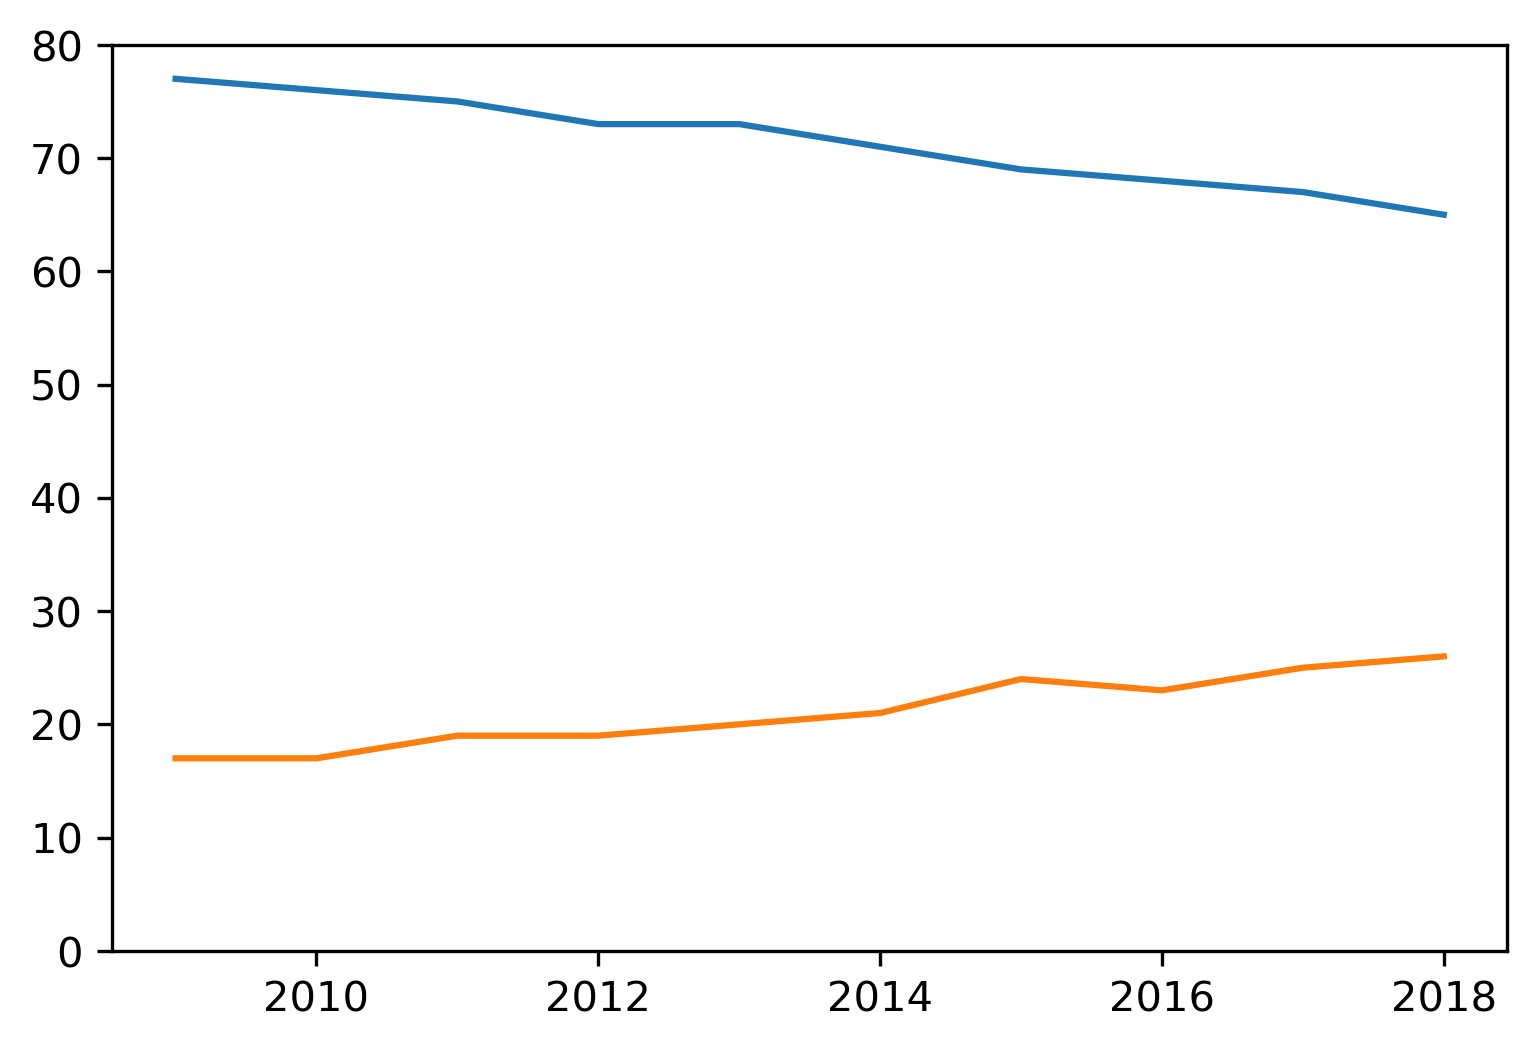
\includegraphics[scale=0.6666666]{06_plotting_files/06_plotting_28_0.png}
\end{center}

The semi-colon at the end of the line prevents the return value from
\passthrough{\lstinline!plot!}, which is an object representing the
line, from being displayed.
\index{semi-colon}

\pagebreak

If you plot multiple lines in a single cell, they appear on the same
axes.

\begin{lstlisting}[language=Python,style=source]
plt.plot(year, christian)
plt.plot(year, unaffiliated);
\end{lstlisting}

\begin{center}
\includegraphics[scale=0.6666666]{06_plotting_files/06_plotting_30_0.png}
\end{center}

Plotting them on the same axes makes it possible to compare them
directly. However, notice that Pyplot chooses the range for the axes
automatically. In this example the y-axis starts around 15, not zero.
\index{axes}

As a result, it provides a misleading picture, making the ratio of the
two lines look bigger than it really is. We can set the limits of the
y-axis using the function \passthrough{\lstinline!plt.ylim!} -- the
arguments are the lower bound and the upper bounds.
\index{ylim (Pyplot function)}

\begin{lstlisting}[language=Python,style=source]
plt.plot(year, christian)
plt.plot(year, unaffiliated)

plt.ylim(0, 80);
\end{lstlisting}

\begin{center}
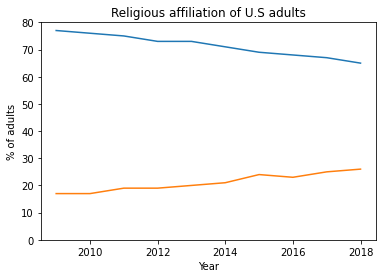
\includegraphics[scale=0.6666666]{06_plotting_files/06_plotting_32_0.png}
\end{center}

That's better, but this graph is missing some important elements: labels
for the axes, a title, and a legend.

\section{Decorating the Axes}\label{decorating-the-axes}

To label the axes and add a title, we'll use Pyplot functions
\passthrough{\lstinline!xlabel!}, \passthrough{\lstinline!ylabel!}, and
\passthrough{\lstinline!title!}. All of them take strings as arguments.
\index{xlabel (Pyplot function)}
\index{ylabel (Pyplot function)}
\index{title (Pyplot function)}

\begin{lstlisting}[language=Python,style=source]
plt.plot(year, christian)
plt.plot(year, unaffiliated)

plt.ylim(0, 80)
plt.xlabel('Year')
plt.ylabel('% of adults')
plt.title('Religious affiliation of U.S adults');
\end{lstlisting}

\begin{center}
\includegraphics[scale=0.6666666]{06_plotting_files/06_plotting_35_0.png}
\end{center}

To add a legend, first we add a label to each line, using the keyword
argument \passthrough{\lstinline!label!}. Then we call
\passthrough{\lstinline!plt.legend!} to create the legend.
\index{legend (Pyplot function)}

\begin{lstlisting}[language=Python,style=source]
plt.plot(year, christian, label='Christian')
plt.plot(year, unaffiliated, label='Unaffiliated')

plt.ylim(0, 80)
plt.xlabel('Year')
plt.ylabel('% of adults')
plt.title('Religious affiliation of U.S adults')
plt.legend();
\end{lstlisting}

\begin{center}
\includegraphics[scale=0.6666666]{06_plotting_files/06_plotting_37_0.png}
\end{center}

The legend shows the labels we provided when we created the lines.

\textbf{Exercise:} The original figure plots lines between the data
points, but it also plots markers showing the location of each data
point. It is good practice to include these markers, especially if data
are not available for every year.

Modify the previous example to include a keyword argument
\passthrough{\lstinline!marker!} with the string value
\passthrough{\lstinline!'.'!}, which indicates that you want to plot
small circles as markers.

\textbf{Exercise:} In the original figure, the line labeled
\passthrough{\lstinline!'Christian'!} is red and the line labeled
\passthrough{\lstinline!'Unaffiliated'!} is gray.

Find the online documentation of \passthrough{\lstinline!plt.plot!}, or
ask a virtual assistant like ChatGPT, and figure out how to use keyword
arguments to specify colors. Choose colors to (roughly) match the
original figure.

The \passthrough{\lstinline!legend!} function takes a keyword argument
that specifies the location of the legend. Read the documentation of
this function and move the legend to the center left of the figure.

\section{Plotting Sandwich Prices}\label{plotting-sandwich-prices}

In Chapter 3 we used data from an article in \emph{The Economist}
comparing sandwich prices in Boston and London: ``Why Americans pay more
for lunch than Britons do''.
\index{The Economist@\textit{The Economist}}
\index{sandwich prices}

\pagebreak

The article includes this graph showing prices of several sandwiches in
the two cities:

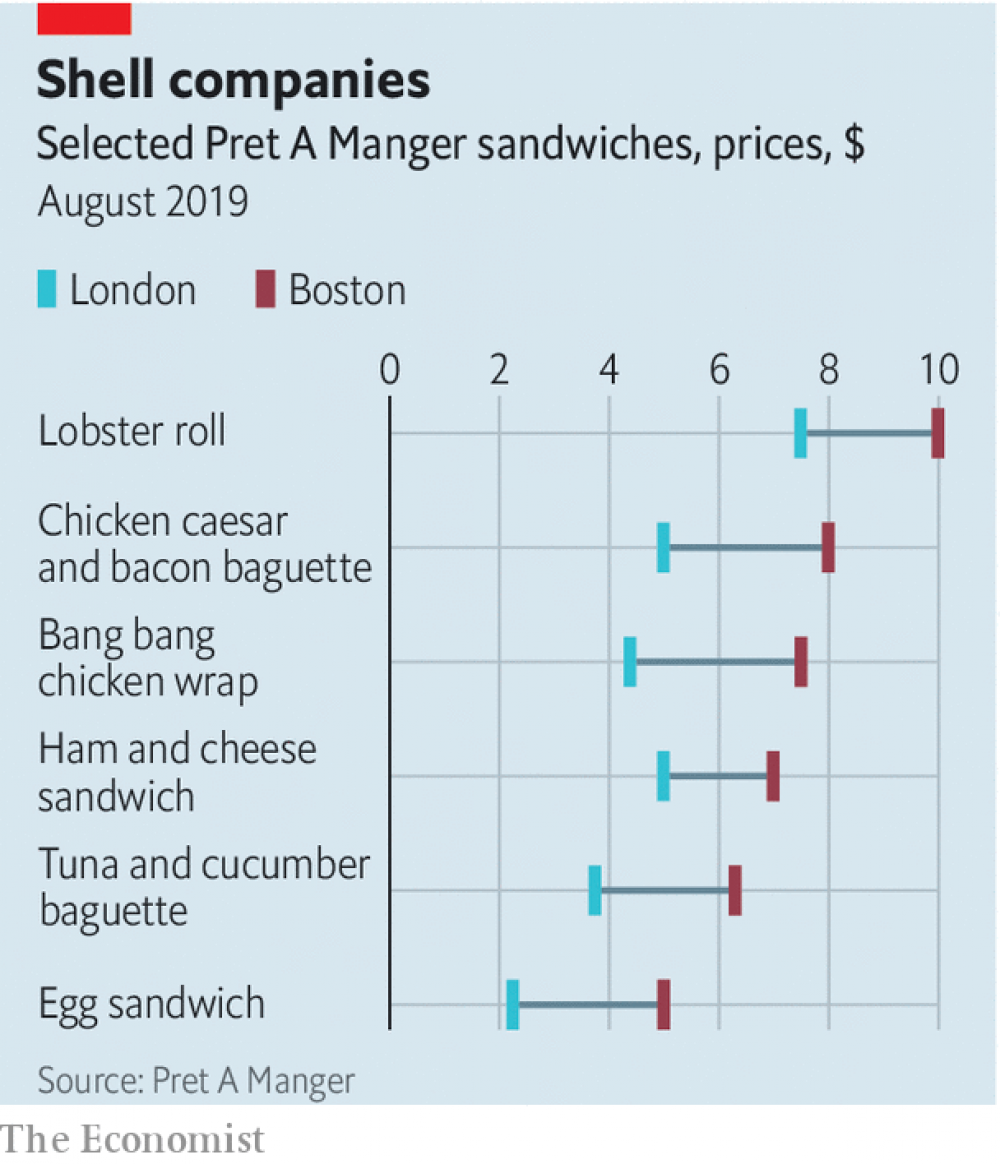
\includegraphics[scale=0.2]{figs/20190907_FNC941.png}

As an exercise, let's see if we can replicate this figure. Here's the
data from the article again.

\begin{lstlisting}[language=Python,style=source]
name_list = [
    'Lobster roll',
    'Chicken caesar',
    'Bang bang chicken',
    'Ham and cheese',
    'Tuna and cucumber',
    'Egg'
]
\end{lstlisting}

\begin{lstlisting}[language=Python,style=source]
boston_price_list = [9.99, 7.99, 7.49, 7, 6.29, 4.99]
london_price_list = [7.5, 5, 4.4, 5, 3.75, 2.25]
\end{lstlisting}

In the previous section we plotted percentages on the y-axis versus time
on the x-axis. Now we want to plot the sandwich names on the y-axis and
the prices on the x-axis. Here's how:

\begin{lstlisting}[language=Python,style=source]
plt.plot(boston_price_list, name_list)
plt.xlabel('Price in USD');
\end{lstlisting}

\begin{center}
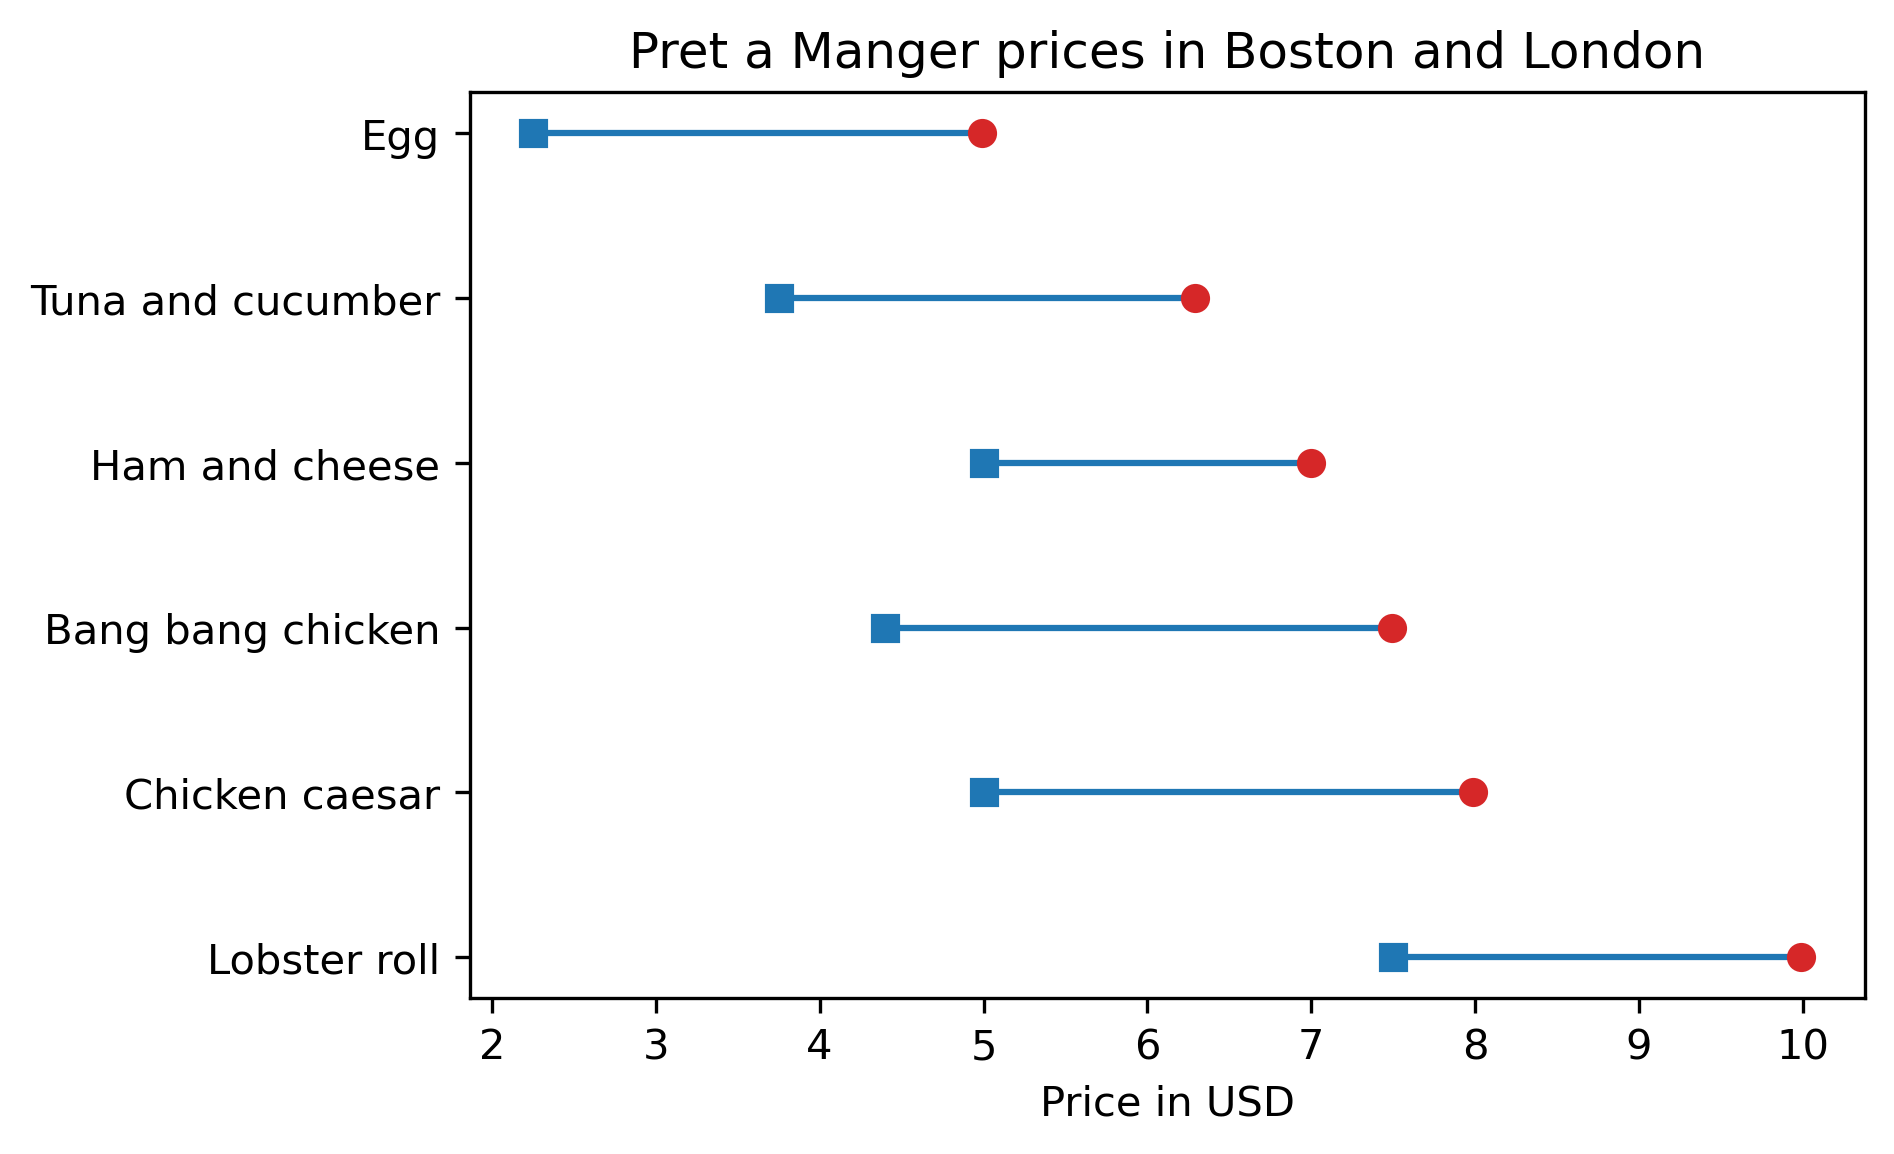
\includegraphics[scale=0.6666666]{06_plotting_files/06_plotting_47_0.png}
\end{center}

By default Pyplot connects the points with lines, but in this example
the lines don't make sense because the sandwich names are discrete --
that is, there are no intermediate points between an egg sandwich and a
tuna sandwich. We can remove the lines and add markers with the keywords
\passthrough{\lstinline!linestyle!} and
\passthrough{\lstinline!marker!}.

\begin{lstlisting}[language=Python,style=source]
plt.plot(boston_price_list, name_list, linestyle='', marker='o')
plt.xlabel('Price in USD');
\end{lstlisting}

\begin{center}
\includegraphics[scale=0.6666666]{06_plotting_files/06_plotting_49_0.png}
\end{center}

Or we can do the same thing more concisely by providing a \textbf{format
string} as a positional argument. In the following examples,
\passthrough{\lstinline!'o'!} indicates a circle marker and
\passthrough{\lstinline!'s'!} indicates a square. You can read the
documentation of \passthrough{\lstinline!plt.plot!} to learn more about
format strings.

\begin{lstlisting}[language=Python,style=source]
plt.plot(boston_price_list, name_list, 'o')
plt.plot(london_price_list, name_list, 's')

plt.xlabel('Price in USD')
plt.title('Pret a Manger prices in Boston and London');
\end{lstlisting}

\begin{center}
\includegraphics[scale=0.6666666]{06_plotting_files/06_plotting_51_0.png}
\end{center}

Now, to approximate the colors in the original figure, we can use the
strings \passthrough{\lstinline!'C3'!} and
\passthrough{\lstinline!'C0'!}, which specify colors from the default
color sequence.
\index{color sequence (Pyplot)}

\begin{lstlisting}[language=Python,style=source]
plt.plot(boston_price_list, name_list, 'o', color='C3')
plt.plot(london_price_list, name_list, 's', color='C0')

plt.xlabel('Price in USD')
plt.title('Pret a Manger prices in Boston and London');
\end{lstlisting}

\begin{center}
\includegraphics[scale=0.6666666]{06_plotting_files/06_plotting_53_0.png}
\end{center}

To connect the dots with lines, we'll use
\passthrough{\lstinline!plt.hlines!}, which draws horizontal lines. It
takes three arguments: a sequence of values on the y-axis, which are the
sandwich names in this example, and two sequences of values on the
x-axis, which are the London prices and Boston prices.
\index{hlines (Pyplot function)}

\pagebreak

\begin{lstlisting}[language=Python,style=source]
plt.hlines(name_list, london_price_list, boston_price_list, color='gray')

plt.plot(boston_price_list, name_list, 'o', color='C3')
plt.plot(london_price_list, name_list, 's', color='C0')

plt.xlabel('Price in USD')
plt.title('Pret a Manger prices in Boston and London');
\end{lstlisting}

\begin{center}
\includegraphics[scale=0.6666666]{06_plotting_files/06_plotting_55_0.png}
\end{center}

\textbf{Exercise:} To finish off this example, add a legend that
identifies the London and Boston prices. Remember that you have to add a
\passthrough{\lstinline!label!} keyword each time you call
\passthrough{\lstinline!plt.plot!}, and then call
\passthrough{\lstinline!plt.legend!}.

Notice that the sandwiches in our figure are in the opposite order of
the sandwiches in the original figure. There is a Pyplot function that
inverts the y-axis; see if you can find it and use it to reverse the
order of the sandwich list.

\section{Zipf's Law}\label{zipfs-law}

In almost any book, in almost any language, if you count the number of
unique words and the number of times each word appears, you will find a
remarkable pattern: the most common word appears twice as often as the
second most common -- at least approximately -- three times as often as
the third most common, and so on.

In general, if we sort the words in descending order of frequency, there
is an inverse relationship between the rank of the words -- first,
second, third, etc. -- and the number of times they appear. This
observation was most famously made by George Kingsley Zipf, so it is
called Zipf's law.
\index{Zipf's law}

\pagebreak

To see if this law holds for the words in \emph{War and Peace}, we'll
make a Zipf plot, which shows:
\index{Zipf plot}

\begin{itemize}
\item
  The frequency of each word on the y-axis, and
\item
  The rank of each word on the x-axis, starting from 1.
\end{itemize}

In the previous chapter, we looped through the book and made a string
that contains all punctuation characters. Here are the results, which we
will need again.

\begin{lstlisting}[language=Python,style=source]
all_punctuation = ',.-:[#]*/“’—‘!?”;()%@'
\end{lstlisting}

The following program reads through the book and makes a dictionary that
maps from each word to the number of times it appears.

\begin{lstlisting}[language=Python,style=source]
fp = open('2600-0.txt')
for line in fp:
    if line.startswith('***'):
        break

unique_words = {}
for line in fp:
    if line.startswith('***'):
        break

    for word in line.split():
        word = word.lower()
        word = word.strip(all_punctuation)
        if word in unique_words:
            unique_words[word] += 1
        else:
            unique_words[word] = 1
\end{lstlisting}

In \passthrough{\lstinline!unique\_words!}, the keys are words and the
values are their frequencies. We can use the
\passthrough{\lstinline!values!} function to get the values from the
dictionary. The result has the type
\passthrough{\lstinline!dict\_values!}:
\index{values (dict function)}

\begin{lstlisting}[language=Python,style=source]
freqs = unique_words.values()
type(freqs)
\end{lstlisting}

\begin{lstlisting}[style=output]
dict_values
\end{lstlisting}

\pagebreak

Before we plot them, we have to sort them, but the
\passthrough{\lstinline!sort!} function doesn't work with
\passthrough{\lstinline!dict\_values!}.
\index{AttributeError}

\begin{lstlisting}[language=Python,style=source]
%%expect AttributeError

freqs.sort()
\end{lstlisting}

\begin{lstlisting}[style=output]
AttributeError: 'dict_values' object has no attribute 'sort'
\end{lstlisting}

We can use \passthrough{\lstinline!list!} to make a list of frequencies:

\begin{lstlisting}[language=Python,style=source]
freq_list = list(unique_words.values())
type(freq_list)
\end{lstlisting}

\begin{lstlisting}[style=output]
list
\end{lstlisting}

And now we can use \passthrough{\lstinline!sort!}. By default it sorts
in ascending order, but we can pass a keyword argument to reverse the
order.
\index{sort (list method)}

\begin{lstlisting}[language=Python,style=source]
freq_list.sort(reverse=True)
\end{lstlisting}

Now, for the ranks, we need a sequence that counts from 1 to
\passthrough{\lstinline!n!}, where \passthrough{\lstinline!n!} is the
number of elements in \passthrough{\lstinline!freq\_list!}. We can use
the \passthrough{\lstinline!range!} function, which returns a value with
type \passthrough{\lstinline!range!}. As a small example, here's the
range from 1 to 5.
\index{range function}

\begin{lstlisting}[language=Python,style=source]
range(1, 5)
\end{lstlisting}

\begin{lstlisting}[style=output]
range(1, 5)
\end{lstlisting}

However, there's a catch. If we use the range to make a list, we see
that ``the range from 1 to 5'' includes 1, but it doesn't include 5.

\begin{lstlisting}[language=Python,style=source]
list(range(1, 5))
\end{lstlisting}

\begin{lstlisting}[style=output]
[1, 2, 3, 4]
\end{lstlisting}

That might seem strange, but it is often more convenient to use
\passthrough{\lstinline!range!} when it is defined this way, rather than
what might seem like the more natural way. Anyway, we can get what we
want by increasing the second argument by one:

\begin{lstlisting}[language=Python,style=source]
list(range(1, 6))
\end{lstlisting}

\begin{lstlisting}[style=output]
[1, 2, 3, 4, 5]
\end{lstlisting}

\pagebreak

So, finally, we can make a range that represents the ranks from
\passthrough{\lstinline!1!} to \passthrough{\lstinline!n!}:
\index{rank}

\begin{lstlisting}[language=Python,style=source]
n = len(freq_list)
ranks = range(1, n+1)
ranks
\end{lstlisting}

\begin{lstlisting}[style=output]
range(1, 20484)
\end{lstlisting}

And now we can plot the frequencies versus the ranks:
\index{frequency}

\begin{lstlisting}[language=Python,style=source]
plt.plot(ranks, freq_list)

plt.xlabel('Rank')
plt.ylabel('Frequency')
plt.title("War and Peace and Zipf's law");
\end{lstlisting}

\begin{center}
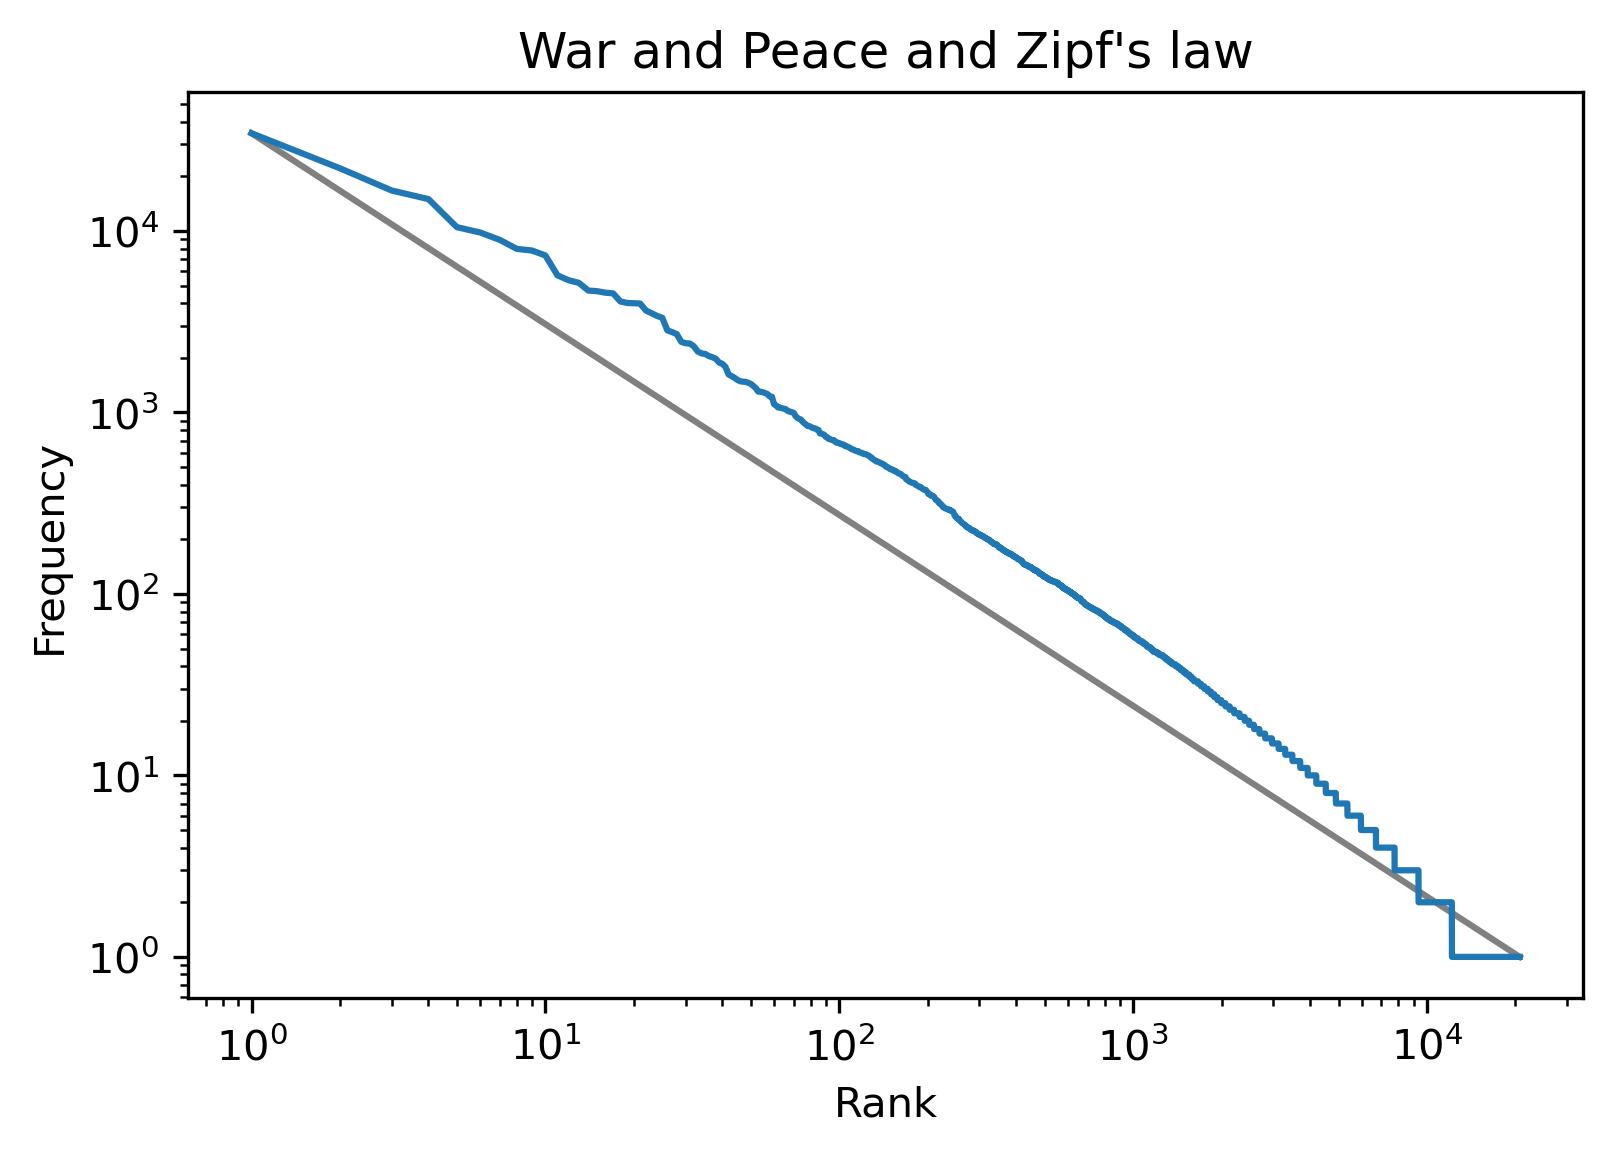
\includegraphics[scale=0.6666666]{06_plotting_files/06_plotting_83_0.png}
\end{center}

According to Zipf's law, these frequencies should be inversely
proportional to the ranks. If that's true, we can write:

\(f = k / r\)

where \(r\) is the rank of a word, \(f\) is its frequency, and \(k\) is
an unknown constant of proportionality. If we take the logarithm of both
sides, we get

\(\log f = \log k - \log r\)

This equation implies that if we plot \(f\) versus \(r\) on a log-log
scale, we expect to see a straight line with intercept at \(\log k\) and
slope \(-1\).

\section{Logarithmic Scales}\label{logarithmic-scales}

We can use \passthrough{\lstinline!plt.xscale!} to plot the x-axis on a
log scale.
\index{logarithmic scale}
\index{xscale (Pyplot function)}

\begin{lstlisting}[language=Python,style=source]
plt.plot(ranks, freq_list)

plt.xlabel('Rank')
plt.ylabel('Frequency')
plt.title("War and Peace and Zipf's law")
plt.xscale('log')
\end{lstlisting}

\begin{center}
\includegraphics[scale=0.6666666]{06_plotting_files/06_plotting_86_0.png}
\end{center}

And \passthrough{\lstinline!plt.yscale!} to plot the y-axis on a log
scale.
\index{yscale (Pyplot function)}

\begin{lstlisting}[language=Python,style=source]
plt.plot(ranks, freq_list)

plt.xlabel('Rank')
plt.ylabel('Frequency')
plt.title("War and Peace and Zipf's law")
plt.xscale('log')
plt.yscale('log')
\end{lstlisting}

\begin{center}
\includegraphics[scale=0.6666666]{06_plotting_files/06_plotting_88_0.png}
\end{center}

The result is not quite a straight line, but it is close. We can get a
sense of the slope by connecting the end points with a line. First,
we'll select the first and last elements from
\passthrough{\lstinline!xs!}.

\begin{lstlisting}[language=Python,style=source]
xs = ranks[0], ranks[-1]
xs
\end{lstlisting}

\begin{lstlisting}[style=output]
(1, 20483)
\end{lstlisting}

And the first and last elements from \passthrough{\lstinline!ys!}.

\begin{lstlisting}[language=Python,style=source]
ys = freq_list[0], freq_list[-1]
ys
\end{lstlisting}

\begin{lstlisting}[style=output]
(34389, 1)
\end{lstlisting}

And plot a line between them.

\begin{lstlisting}[language=Python,style=source]
plt.plot(xs, ys, color='gray')
plt.plot(ranks, freq_list)

plt.xlabel('Rank')
plt.ylabel('Frequency')
plt.title("War and Peace and Zipf's law")
plt.xscale('log')
plt.yscale('log')
\end{lstlisting}

\begin{center}
\includegraphics[scale=0.6666666]{06_plotting_files/06_plotting_94_0.png}
\end{center}

The slope of this line is the ``rise over run'', that is, the difference
on the y-axis divided by the difference on the x-axis. We can compute
the rise using \passthrough{\lstinline!np.log10!} to compute the log
base 10 of the first and last values:
\index{slope of a line}
\index{rise over run}

\begin{lstlisting}[language=Python,style=source]
np.log10(ys)
\end{lstlisting}

\begin{lstlisting}[style=output]
array([4.53641955, 0.        ])
\end{lstlisting}

Then we can use \passthrough{\lstinline!np.diff!} to compute the
difference between the elements:

\begin{lstlisting}[language=Python,style=source]
rise = np.diff(np.log10(ys))
rise
\end{lstlisting}

\begin{lstlisting}[style=output]
array([-4.53641955])
\end{lstlisting}

\textbf{Exercise:} Use \passthrough{\lstinline!log10!} and
\passthrough{\lstinline!diff!} to compute the run, that is, the
difference on the x-axis. Then divide the rise by the run to get the
slope of the grey line. Is it close to \(-1\), as Zipf's law predicts?

\section{Summary}\label{summary}

This chapter introduces Pyplot, which is part of the Matplotlib library.
We used to replicate two figures and make a Zipf plot. These examples
demonstrate the most common elements of data visualization, including
lines and markers, values and labels on the axes, a legend and a title.
The Zipf plot also shows the power of plotting data on logarithmic
scales.
